\documentclass{article} % For LaTeX2e
\usepackage{iclr2022_conference,times}
% Optional math commands from https://github.com/goodfeli/dlbook_notation.
%%%%% NEW MATH DEFINITIONS %%%%%

\usepackage{amsmath,amsfonts,bm}

% Mark sections of captions for referring to divisions of figures
\newcommand{\figleft}{{\em (Left)}}
\newcommand{\figcenter}{{\em (Center)}}
\newcommand{\figright}{{\em (Right)}}
\newcommand{\figtop}{{\em (Top)}}
\newcommand{\figbottom}{{\em (Bottom)}}
\newcommand{\captiona}{{\em (a)}}
\newcommand{\captionb}{{\em (b)}}
\newcommand{\captionc}{{\em (c)}}
\newcommand{\captiond}{{\em (d)}}

% Highlight a newly defined term
\newcommand{\newterm}[1]{{\bf #1}}


% Figure reference, lower-case.
\def\figref#1{figure~\ref{#1}}
% Figure reference, capital. For start of sentence
\def\Figref#1{Figure~\ref{#1}}
\def\twofigref#1#2{figures \ref{#1} and \ref{#2}}
\def\quadfigref#1#2#3#4{figures \ref{#1}, \ref{#2}, \ref{#3} and \ref{#4}}
% Section reference, lower-case.
\def\secref#1{section~\ref{#1}}
% Section reference, capital.
\def\Secref#1{Section~\ref{#1}}
% Reference to two sections.
\def\twosecrefs#1#2{sections \ref{#1} and \ref{#2}}
% Reference to three sections.
\def\secrefs#1#2#3{sections \ref{#1}, \ref{#2} and \ref{#3}}
% Reference to an equation, lower-case.
\def\eqref#1{equation~\ref{#1}}
% Reference to an equation, upper case
\def\Eqref#1{Equation~\ref{#1}}
% A raw reference to an equation---avoid using if possible
\def\plaineqref#1{\ref{#1}}
% Reference to a chapter, lower-case.
\def\chapref#1{chapter~\ref{#1}}
% Reference to an equation, upper case.
\def\Chapref#1{Chapter~\ref{#1}}
% Reference to a range of chapters
\def\rangechapref#1#2{chapters\ref{#1}--\ref{#2}}
% Reference to an algorithm, lower-case.
\def\algref#1{algorithm~\ref{#1}}
% Reference to an algorithm, upper case.
\def\Algref#1{Algorithm~\ref{#1}}
\def\twoalgref#1#2{algorithms \ref{#1} and \ref{#2}}
\def\Twoalgref#1#2{Algorithms \ref{#1} and \ref{#2}}
% Reference to a part, lower case
\def\partref#1{part~\ref{#1}}
% Reference to a part, upper case
\def\Partref#1{Part~\ref{#1}}
\def\twopartref#1#2{parts \ref{#1} and \ref{#2}}

\def\ceil#1{\lceil #1 \rceil}
\def\floor#1{\lfloor #1 \rfloor}
\def\1{\bm{1}}
\newcommand{\train}{\mathcal{D}}
\newcommand{\valid}{\mathcal{D_{\mathrm{valid}}}}
\newcommand{\test}{\mathcal{D_{\mathrm{test}}}}

\def\eps{{\epsilon}}


% Random variables
\def\reta{{\textnormal{$\eta$}}}
\def\ra{{\textnormal{a}}}
\def\rb{{\textnormal{b}}}
\def\rc{{\textnormal{c}}}
\def\rd{{\textnormal{d}}}
\def\re{{\textnormal{e}}}
\def\rf{{\textnormal{f}}}
\def\rg{{\textnormal{g}}}
\def\rh{{\textnormal{h}}}
\def\ri{{\textnormal{i}}}
\def\rj{{\textnormal{j}}}
\def\rk{{\textnormal{k}}}
\def\rl{{\textnormal{l}}}
% rm is already a command, just don't name any random variables m
\def\rn{{\textnormal{n}}}
\def\ro{{\textnormal{o}}}
\def\rp{{\textnormal{p}}}
\def\rq{{\textnormal{q}}}
\def\rr{{\textnormal{r}}}
\def\rs{{\textnormal{s}}}
\def\rt{{\textnormal{t}}}
\def\ru{{\textnormal{u}}}
\def\rv{{\textnormal{v}}}
\def\rw{{\textnormal{w}}}
\def\rx{{\textnormal{x}}}
\def\ry{{\textnormal{y}}}
\def\rz{{\textnormal{z}}}

% Random vectors
\def\rvepsilon{{\mathbf{\epsilon}}}
\def\rvtheta{{\mathbf{\theta}}}
\def\rva{{\mathbf{a}}}
\def\rvb{{\mathbf{b}}}
\def\rvc{{\mathbf{c}}}
\def\rvd{{\mathbf{d}}}
\def\rve{{\mathbf{e}}}
\def\rvf{{\mathbf{f}}}
\def\rvg{{\mathbf{g}}}
\def\rvh{{\mathbf{h}}}
\def\rvu{{\mathbf{i}}}
\def\rvj{{\mathbf{j}}}
\def\rvk{{\mathbf{k}}}
\def\rvl{{\mathbf{l}}}
\def\rvm{{\mathbf{m}}}
\def\rvn{{\mathbf{n}}}
\def\rvo{{\mathbf{o}}}
\def\rvp{{\mathbf{p}}}
\def\rvq{{\mathbf{q}}}
\def\rvr{{\mathbf{r}}}
\def\rvs{{\mathbf{s}}}
\def\rvt{{\mathbf{t}}}
\def\rvu{{\mathbf{u}}}
\def\rvv{{\mathbf{v}}}
\def\rvw{{\mathbf{w}}}
\def\rvx{{\mathbf{x}}}
\def\rvy{{\mathbf{y}}}
\def\rvz{{\mathbf{z}}}

% Elements of random vectors
\def\erva{{\textnormal{a}}}
\def\ervb{{\textnormal{b}}}
\def\ervc{{\textnormal{c}}}
\def\ervd{{\textnormal{d}}}
\def\erve{{\textnormal{e}}}
\def\ervf{{\textnormal{f}}}
\def\ervg{{\textnormal{g}}}
\def\ervh{{\textnormal{h}}}
\def\ervi{{\textnormal{i}}}
\def\ervj{{\textnormal{j}}}
\def\ervk{{\textnormal{k}}}
\def\ervl{{\textnormal{l}}}
\def\ervm{{\textnormal{m}}}
\def\ervn{{\textnormal{n}}}
\def\ervo{{\textnormal{o}}}
\def\ervp{{\textnormal{p}}}
\def\ervq{{\textnormal{q}}}
\def\ervr{{\textnormal{r}}}
\def\ervs{{\textnormal{s}}}
\def\ervt{{\textnormal{t}}}
\def\ervu{{\textnormal{u}}}
\def\ervv{{\textnormal{v}}}
\def\ervw{{\textnormal{w}}}
\def\ervx{{\textnormal{x}}}
\def\ervy{{\textnormal{y}}}
\def\ervz{{\textnormal{z}}}

% Random matrices
\def\rmA{{\mathbf{A}}}
\def\rmB{{\mathbf{B}}}
\def\rmC{{\mathbf{C}}}
\def\rmD{{\mathbf{D}}}
\def\rmE{{\mathbf{E}}}
\def\rmF{{\mathbf{F}}}
\def\rmG{{\mathbf{G}}}
\def\rmH{{\mathbf{H}}}
\def\rmI{{\mathbf{I}}}
\def\rmJ{{\mathbf{J}}}
\def\rmK{{\mathbf{K}}}
\def\rmL{{\mathbf{L}}}
\def\rmM{{\mathbf{M}}}
\def\rmN{{\mathbf{N}}}
\def\rmO{{\mathbf{O}}}
\def\rmP{{\mathbf{P}}}
\def\rmQ{{\mathbf{Q}}}
\def\rmR{{\mathbf{R}}}
\def\rmS{{\mathbf{S}}}
\def\rmT{{\mathbf{T}}}
\def\rmU{{\mathbf{U}}}
\def\rmV{{\mathbf{V}}}
\def\rmW{{\mathbf{W}}}
\def\rmX{{\mathbf{X}}}
\def\rmY{{\mathbf{Y}}}
\def\rmZ{{\mathbf{Z}}}

% Elements of random matrices
\def\ermA{{\textnormal{A}}}
\def\ermB{{\textnormal{B}}}
\def\ermC{{\textnormal{C}}}
\def\ermD{{\textnormal{D}}}
\def\ermE{{\textnormal{E}}}
\def\ermF{{\textnormal{F}}}
\def\ermG{{\textnormal{G}}}
\def\ermH{{\textnormal{H}}}
\def\ermI{{\textnormal{I}}}
\def\ermJ{{\textnormal{J}}}
\def\ermK{{\textnormal{K}}}
\def\ermL{{\textnormal{L}}}
\def\ermM{{\textnormal{M}}}
\def\ermN{{\textnormal{N}}}
\def\ermO{{\textnormal{O}}}
\def\ermP{{\textnormal{P}}}
\def\ermQ{{\textnormal{Q}}}
\def\ermR{{\textnormal{R}}}
\def\ermS{{\textnormal{S}}}
\def\ermT{{\textnormal{T}}}
\def\ermU{{\textnormal{U}}}
\def\ermV{{\textnormal{V}}}
\def\ermW{{\textnormal{W}}}
\def\ermX{{\textnormal{X}}}
\def\ermY{{\textnormal{Y}}}
\def\ermZ{{\textnormal{Z}}}

% Vectors
\def\vzero{{\bm{0}}}
\def\vone{{\bm{1}}}
\def\vmu{{\bm{\mu}}}
\def\vtheta{{\bm{\theta}}}
\def\va{{\bm{a}}}
\def\vb{{\bm{b}}}
\def\vc{{\bm{c}}}
\def\vd{{\bm{d}}}
\def\ve{{\bm{e}}}
\def\vf{{\bm{f}}}
\def\vg{{\bm{g}}}
\def\vh{{\bm{h}}}
\def\vi{{\bm{i}}}
\def\vj{{\bm{j}}}
\def\vk{{\bm{k}}}
\def\vl{{\bm{l}}}
\def\vm{{\bm{m}}}
\def\vn{{\bm{n}}}
\def\vo{{\bm{o}}}
\def\vp{{\bm{p}}}
\def\vq{{\bm{q}}}
\def\vr{{\bm{r}}}
\def\vs{{\bm{s}}}
\def\vt{{\bm{t}}}
\def\vu{{\bm{u}}}
\def\vv{{\bm{v}}}
\def\vw{{\bm{w}}}
\def\vx{{\bm{x}}}
\def\vy{{\bm{y}}}
\def\vz{{\bm{z}}}

% Elements of vectors
\def\evalpha{{\alpha}}
\def\evbeta{{\beta}}
\def\evepsilon{{\epsilon}}
\def\evlambda{{\lambda}}
\def\evomega{{\omega}}
\def\evmu{{\mu}}
\def\evpsi{{\psi}}
\def\evsigma{{\sigma}}
\def\evtheta{{\theta}}
\def\eva{{a}}
\def\evb{{b}}
\def\evc{{c}}
\def\evd{{d}}
\def\eve{{e}}
\def\evf{{f}}
\def\evg{{g}}
\def\evh{{h}}
\def\evi{{i}}
\def\evj{{j}}
\def\evk{{k}}
\def\evl{{l}}
\def\evm{{m}}
\def\evn{{n}}
\def\evo{{o}}
\def\evp{{p}}
\def\evq{{q}}
\def\evr{{r}}
\def\evs{{s}}
\def\evt{{t}}
\def\evu{{u}}
\def\evv{{v}}
\def\evw{{w}}
\def\evx{{x}}
\def\evy{{y}}
\def\evz{{z}}

% Matrix
\def\mA{{\bm{A}}}
\def\mB{{\bm{B}}}
\def\mC{{\bm{C}}}
\def\mD{{\bm{D}}}
\def\mE{{\bm{E}}}
\def\mF{{\bm{F}}}
\def\mG{{\bm{G}}}
\def\mH{{\bm{H}}}
\def\mI{{\bm{I}}}
\def\mJ{{\bm{J}}}
\def\mK{{\bm{K}}}
\def\mL{{\bm{L}}}
\def\mM{{\bm{M}}}
\def\mN{{\bm{N}}}
\def\mO{{\bm{O}}}
\def\mP{{\bm{P}}}
\def\mQ{{\bm{Q}}}
\def\mR{{\bm{R}}}
\def\mS{{\bm{S}}}
\def\mT{{\bm{T}}}
\def\mU{{\bm{U}}}
\def\mV{{\bm{V}}}
\def\mW{{\bm{W}}}
\def\mX{{\bm{X}}}
\def\mY{{\bm{Y}}}
\def\mZ{{\bm{Z}}}
\def\mBeta{{\bm{\beta}}}
\def\mPhi{{\bm{\Phi}}}
\def\mLambda{{\bm{\Lambda}}}
\def\mSigma{{\bm{\Sigma}}}

% Tensor
\DeclareMathAlphabet{\mathsfit}{\encodingdefault}{\sfdefault}{m}{sl}
\SetMathAlphabet{\mathsfit}{bold}{\encodingdefault}{\sfdefault}{bx}{n}
\newcommand{\tens}[1]{\bm{\mathsfit{#1}}}
\def\tA{{\tens{A}}}
\def\tB{{\tens{B}}}
\def\tC{{\tens{C}}}
\def\tD{{\tens{D}}}
\def\tE{{\tens{E}}}
\def\tF{{\tens{F}}}
\def\tG{{\tens{G}}}
\def\tH{{\tens{H}}}
\def\tI{{\tens{I}}}
\def\tJ{{\tens{J}}}
\def\tK{{\tens{K}}}
\def\tL{{\tens{L}}}
\def\tM{{\tens{M}}}
\def\tN{{\tens{N}}}
\def\tO{{\tens{O}}}
\def\tP{{\tens{P}}}
\def\tQ{{\tens{Q}}}
\def\tR{{\tens{R}}}
\def\tS{{\tens{S}}}
\def\tT{{\tens{T}}}
\def\tU{{\tens{U}}}
\def\tV{{\tens{V}}}
\def\tW{{\tens{W}}}
\def\tX{{\tens{X}}}
\def\tY{{\tens{Y}}}
\def\tZ{{\tens{Z}}}


% Graph
\def\gA{{\mathcal{A}}}
\def\gB{{\mathcal{B}}}
\def\gC{{\mathcal{C}}}
\def\gD{{\mathcal{D}}}
\def\gE{{\mathcal{E}}}
\def\gF{{\mathcal{F}}}
\def\gG{{\mathcal{G}}}
\def\gH{{\mathcal{H}}}
\def\gI{{\mathcal{I}}}
\def\gJ{{\mathcal{J}}}
\def\gK{{\mathcal{K}}}
\def\gL{{\mathcal{L}}}
\def\gM{{\mathcal{M}}}
\def\gN{{\mathcal{N}}}
\def\gO{{\mathcal{O}}}
\def\gP{{\mathcal{P}}}
\def\gQ{{\mathcal{Q}}}
\def\gR{{\mathcal{R}}}
\def\gS{{\mathcal{S}}}
\def\gT{{\mathcal{T}}}
\def\gU{{\mathcal{U}}}
\def\gV{{\mathcal{V}}}
\def\gW{{\mathcal{W}}}
\def\gX{{\mathcal{X}}}
\def\gY{{\mathcal{Y}}}
\def\gZ{{\mathcal{Z}}}

% Sets
\def\sA{{\mathbb{A}}}
\def\sB{{\mathbb{B}}}
\def\sC{{\mathbb{C}}}
\def\sD{{\mathbb{D}}}
% Don't use a set called E, because this would be the same as our symbol
% for expectation.
\def\sF{{\mathbb{F}}}
\def\sG{{\mathbb{G}}}
\def\sH{{\mathbb{H}}}
\def\sI{{\mathbb{I}}}
\def\sJ{{\mathbb{J}}}
\def\sK{{\mathbb{K}}}
\def\sL{{\mathbb{L}}}
\def\sM{{\mathbb{M}}}
\def\sN{{\mathbb{N}}}
\def\sO{{\mathbb{O}}}
\def\sP{{\mathbb{P}}}
\def\sQ{{\mathbb{Q}}}
\def\sR{{\mathbb{R}}}
\def\sS{{\mathbb{S}}}
\def\sT{{\mathbb{T}}}
\def\sU{{\mathbb{U}}}
\def\sV{{\mathbb{V}}}
\def\sW{{\mathbb{W}}}
\def\sX{{\mathbb{X}}}
\def\sY{{\mathbb{Y}}}
\def\sZ{{\mathbb{Z}}}

% Entries of a matrix
\def\emLambda{{\Lambda}}
\def\emA{{A}}
\def\emB{{B}}
\def\emC{{C}}
\def\emD{{D}}
\def\emE{{E}}
\def\emF{{F}}
\def\emG{{G}}
\def\emH{{H}}
\def\emI{{I}}
\def\emJ{{J}}
\def\emK{{K}}
\def\emL{{L}}
\def\emM{{M}}
\def\emN{{N}}
\def\emO{{O}}
\def\emP{{P}}
\def\emQ{{Q}}
\def\emR{{R}}
\def\emS{{S}}
\def\emT{{T}}
\def\emU{{U}}
\def\emV{{V}}
\def\emW{{W}}
\def\emX{{X}}
\def\emY{{Y}}
\def\emZ{{Z}}
\def\emSigma{{\Sigma}}

% entries of a tensor
% Same font as tensor, without \bm wrapper
\newcommand{\etens}[1]{\mathsfit{#1}}
\def\etLambda{{\etens{\Lambda}}}
\def\etA{{\etens{A}}}
\def\etB{{\etens{B}}}
\def\etC{{\etens{C}}}
\def\etD{{\etens{D}}}
\def\etE{{\etens{E}}}
\def\etF{{\etens{F}}}
\def\etG{{\etens{G}}}
\def\etH{{\etens{H}}}
\def\etI{{\etens{I}}}
\def\etJ{{\etens{J}}}
\def\etK{{\etens{K}}}
\def\etL{{\etens{L}}}
\def\etM{{\etens{M}}}
\def\etN{{\etens{N}}}
\def\etO{{\etens{O}}}
\def\etP{{\etens{P}}}
\def\etQ{{\etens{Q}}}
\def\etR{{\etens{R}}}
\def\etS{{\etens{S}}}
\def\etT{{\etens{T}}}
\def\etU{{\etens{U}}}
\def\etV{{\etens{V}}}
\def\etW{{\etens{W}}}
\def\etX{{\etens{X}}}
\def\etY{{\etens{Y}}}
\def\etZ{{\etens{Z}}}

% The true underlying data generating distribution
\newcommand{\pdata}{p_{\rm{data}}}
% The empirical distribution defined by the training set
\newcommand{\ptrain}{\hat{p}_{\rm{data}}}
\newcommand{\Ptrain}{\hat{P}_{\rm{data}}}
% The model distribution
\newcommand{\pmodel}{p_{\rm{model}}}
\newcommand{\Pmodel}{P_{\rm{model}}}
\newcommand{\ptildemodel}{\tilde{p}_{\rm{model}}}
% Stochastic autoencoder distributions
\newcommand{\pencode}{p_{\rm{encoder}}}
\newcommand{\pdecode}{p_{\rm{decoder}}}
\newcommand{\precons}{p_{\rm{reconstruct}}}

\newcommand{\laplace}{\mathrm{Laplace}} % Laplace distribution

\newcommand{\E}{\mathbb{E}}
\newcommand{\Ls}{\mathcal{L}}
\newcommand{\R}{\mathbb{R}}
\newcommand{\emp}{\tilde{p}}
\newcommand{\lr}{\alpha}
\newcommand{\reg}{\lambda}
\newcommand{\rect}{\mathrm{rectifier}}
\newcommand{\softmax}{\mathrm{softmax}}
\newcommand{\sigmoid}{\sigma}
\newcommand{\softplus}{\zeta}
\newcommand{\KL}{D_{\mathrm{KL}}}
\newcommand{\Var}{\mathrm{Var}}
\newcommand{\standarderror}{\mathrm{SE}}
\newcommand{\Cov}{\mathrm{Cov}}
% Wolfram Mathworld says $L^2$ is for function spaces and $\ell^2$ is for vectors
% But then they seem to use $L^2$ for vectors throughout the site, and so does
% wikipedia.
\newcommand{\normlzero}{L^0}
\newcommand{\normlone}{L^1}
\newcommand{\normltwo}{L^2}
\newcommand{\normlp}{L^p}
\newcommand{\normmax}{L^\infty}

\newcommand{\parents}{Pa} % See usage in notation.tex. Chosen to match Daphne's book.

\DeclareMathOperator*{\argmax}{arg\,max}
\DeclareMathOperator*{\argmin}{arg\,min}

\DeclareMathOperator{\sign}{sign}
\DeclareMathOperator{\Tr}{Tr}
\let\ab\allowbreak


%######## APS360: Uncomment your submission name
%\newcommand{\apsname}{Project Proposal}
\newcommand{\apsname}{Progress Report}
%\newcommand{\apsname}{Final Report}

%######## APS360: Put your Group Number here
\newcommand{\gpnumber}{35}

\usepackage{hyperref}
\usepackage{url}
\usepackage{graphicx}
\usepackage{float} % Add this line in your preamble


%######## APS360: Put your project Title here
\title{Creating a Player Aid for Geometry Dash  \\ 
APS360 Progress Report}


%######## APS360: Put your names, student IDs and Emails here
\author{Jaden Dai \\
Student\# 1009972228\\
\texttt{jaden.dai@mail.utoronto.ca} \\
\And
Joel Vadakken  \\
Student\# 10010089798\\
\texttt{j.vadakken@mail.utoronto.ca} \\
\And
Skyler Han  \\
Student\# 1009794830 \\
\texttt{hs.han@mail.utoronto.ca} \\
\AND
Ian Lu  \\
Student\# 1009972139 \\
\texttt{i.lu@mail.utoronto.ca} \\
\AND
}

% The \author macro works with any number of authors. There are two commands
% used to separate the names and addresses of multiple authors: \And and \AND.
%
% Using \And between authors leaves it to \LaTeX{} to determine where to break
% the lines. Using \AND forces a linebreak at that point. So, if \LaTeX{}
% puts 3 of 4 authors names on the first line, and the last on the second
% line, try using \AND instead of \And before the third author name.

\newcommand{\fix}{\marginpar{FIX}}
\newcommand{\new}{\marginpar{NEW}}

\iclrfinalcopy 
%######## APS360: Document starts here
\begin{document}


\maketitle

\begin{abstract}
Our team intends to create a program that can create semantic segmentation
maps of a Geometry Dash Level using machine learning. This program can be
used to assist players in recognizing obstacles without the usage of mods.
We are using transfer learning to achieve this task.
%######## APS360: Do not change the next line. This shows your Main body page count.
----Total Pages: \pageref{last_page}
\end{abstract}



\section{Brief Project Description}


The goal of our project is to develop a model that takes a screenshot from the game “Geometry Dash” and detects the location of collision boxes automatically. For example, given a live screenshot of the game, it should be able to recognize objects and determine their appropriate collision box:



Above is an example of our desired output for a given screenshot input. Note that Geometry Dash collision boxes are somewhat strangely-shaped, especially for spike objects.

We believe this project is appropriate for deep learning due to the many complexities and edge cases that may appear. For instance, there are many decorative objects that a player can recognize as irrelevant, but may trick a traditional hard-coded or image matching algorithm.


%\begin{figure}[!h]
%\begin{center}
%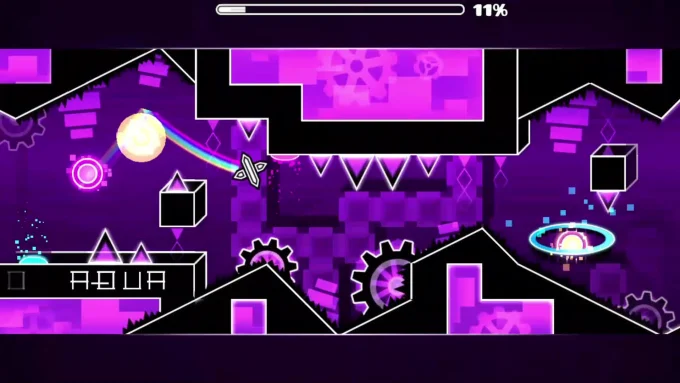
\includegraphics[width=0.6\textwidth]{Figs/example_confusing_image.png}
%\end{center}
%\caption{An example of a level where a mechanism might get confused labelling objects.}
%\label{fig:Confusion_example}
%\end{figure}
 
Here, a player can tell the squares are part of the background, while a hardcoded model may mistake it for a foreground object.

We believe this model could be a useful tool for players, who may not have access to other paid tools to view collision boxes. Furthermore, this may be a useful model for future work in training a RL model to play Geometry Dash by simplifying inputted information.


\section{Individual Contributions and Responsibilities}
\label{gen_inst}

Our team is working well together. We are using github to share code and the latex document, and google docs to share documents for rough work, brainstorming, rough drafts, and data collection. Please see Table \ref{table:contributions} for the tasks we have completed so far. The remaining work we have includes: collecting more data, creating a test set, trying out different architectures, and hyperparameter tuning.  Please see Table \ref{} for how we have decided to divide up these tasks and their deadlines. Since hyperparameter tuning, trying out different architectures, and creating a testset. 

\begin{table}[h]
\caption{Individual Contributions and Tasks}
\label{table:contributions}
\begin{center}
\begin{tabular}{|p{2cm}|p{6cm}|p{6cm}|}
\hline
\multicolumn{1}{|c|}{\bf NAME} & \multicolumn{1}{c|}{\bf CONTRIBUTIONS} & \multicolumn{1}{c|}{\bf TASKS}\\ \hline
Jaden Dai & Did most of the data collection, including creating macros for Geometry Dash levels, creating texture packs, and creating macros for taking screenshots. & Testset creation. Hyperparameter tuning.\\ \hline
Joel Vadakken & Helped with the data collection. Wrote the code to preprocess the data before training the model. & More Data collection. Experiment with different models.\\ \hline
Skyler Han & Created the Baseline model for comparison. Wrote the training code for the model. & Improve baseline model. Experiment with different model architectures\\ \hline 
Ian Lu & Created the architecture for the model, and did some hyperparameter tuning. & Hyperparameter tuning. Testset creation. \\ \hline
\end{tabular}
\end{center}
\end{table}


\begin{table}[h]
\caption{Task Deadlines}
\label{table:task deadlines}
\begin{center}
\begin{tabular}{|p{3cm}|p{3cm}|p{6cm}|}
\hline
\multicolumn{1}{|c|}{\bf TASK} & \multicolumn{1}{c|}{\bf DEADLINE} & \multicolumn{1}{c|}{\bf JUSTIFICATION}\\ \hline
Collecting more data & July 13, 2024 & We need most of our data ready to train our models, so it important we have all of our data ready by then. \\ \hline 
Creating a test set & July 20, 2024 & We won't need to evaluate our model until closer to the submission deadline, so this is not as high priority a task \\ \hline 
Trying out different architectures & July 20, 2024 & We should be done most of our model training so that we can work on our final submission \\ \hline
Hyperparameter tuning & July 20, 2024 & Hyperparameter tuning and trying out different architectures should occur simultaneously, as they are linked together. \\ \hline
\end{tabular}
\end{center}
\end{table}

\section{Data Processing}

We have collected a set of preliminary data directly from the game. The data consists of a live game screenshot with a paired screenshot with labels. See Fig. \ref{fig:sample_data.png}

\begin{figure}[!h]
\begin{center}
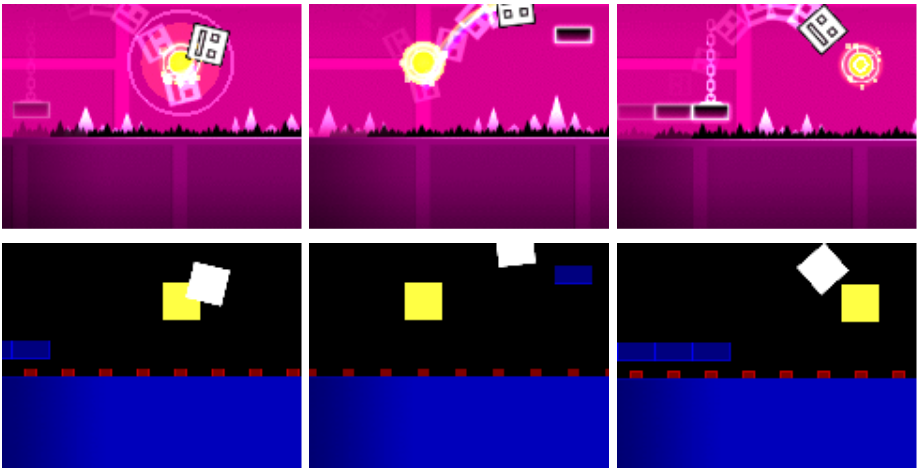
\includegraphics[width=0.6\textwidth]{Figs/sample_data.png}
\end{center}
\caption{3 sample paired screenshots. Top: live screenshot from game. Bottom: labeled screenshots.}
\label{fig:sample_data.png}
\end{figure}

	These screenshots were taken from version 2.1 using the MegaHack V7.1 mod, which features several useful tools (ie. a bot/“macro” to play through levels, a filter for non-gameplay elements). Our exact method is as follows. The exact method is as follows:

\begin{itemize}
    \item Set the game to 1920x1440 resolution with low textures.
    \item Record a “macro” using the built-in MegaHack tool.
    \item Turn on “frame stepper” in MegaHack.
    \item Use a Python script to step through the macro frame-by-frame and take screenshots.
    \begin{itemize}
        \item The bot takes a screenshot every 50 frames, but this can be adjusted.
    \end{itemize}
    \item Load our self-created texture pack by importing files into the game’s directory.
    \item Turn off all visual effects using MegaHack.
    \begin{itemize}
        \item Orb rings, particles, gravity effects, etc.
    \end{itemize}
    \item Enable “Show Layout,” set background to black and ground color to white.
    \item Enable “Show Hitboxes”, set opacity to 100, enable fill, disable player and special hitboxes.
    \item Use the Python script again to take screenshots, which produces the labeled screenshots.
\end{itemize}


Then, from these preliminary labeled screenshots, we further process the data into what can be seen in Fig \ref{fig:labels after post processing}

\begin{figure}[!h]
\begin{center}
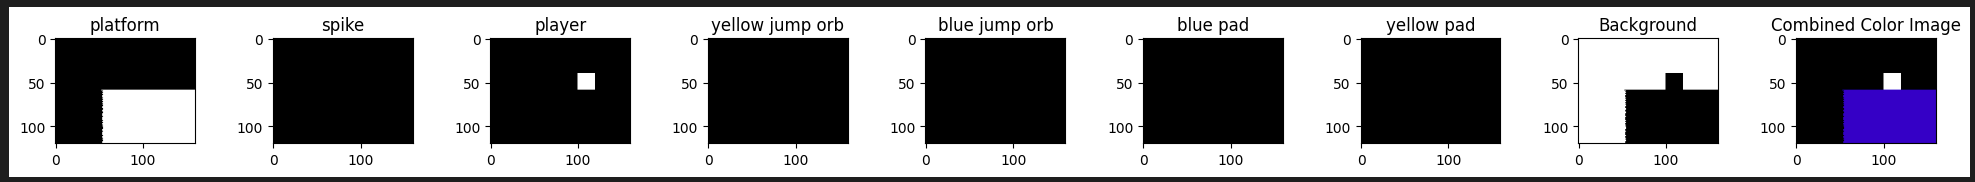
\includegraphics[width=0.6\textwidth]{Figs/labels after post processing.png}
\end{center}
\caption{Post processed data featuring label masks for each class of object.}
\label{fig:labels after post processing}
\end{figure}


Since each class already has its own color, we can then transform this into our dataset by reading in the pixel RGB values and mapping that to a multi-channel mask. Each respective channel represents a specific type of object, which can be seen above. This output data is then used to train our semantic segmentation model.

There were some challenges that we encountered during this process:
The newest version of Geometry Dash (2.2) does not have some tools that are necessary to generate labeled screenshots. For instance, it lacks the ability to “step through frames” which is essential for creating paired screenshots. We attempted some other methods of pausing the game and taking screenshots with some post processing methods, but these methods generated messier and worse data.
Since we used a texture pack, the collision box labels for “orbs” were inaccurate, as the collision box stretches beyond the size of the textures.

\begin{figure}[!h]
\begin{center}
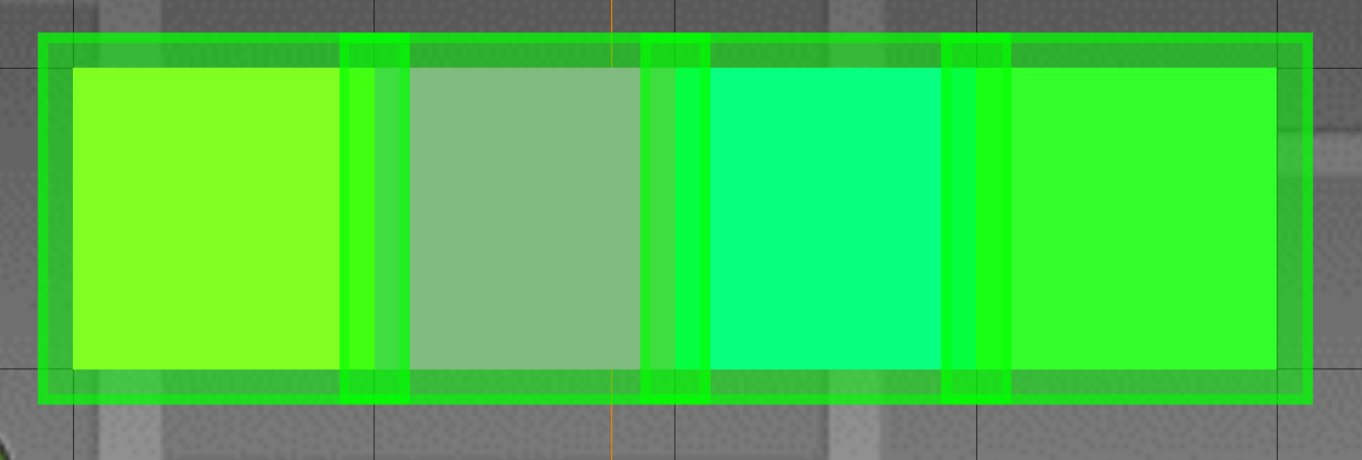
\includegraphics[width=0.6\textwidth]{Figs/collision_box_issues.png}
\end{center}
\caption{Green: Collision box: Inner square: Largest possible label for orb using texture pack}
\label{fig:collision_box_issues}
\end{figure}


This means our final result will be slightly inaccurate.

Most of these challenges could be remedied through the use of a custom-built mod for the game. However, given that this would require learning to inject C++ code, we decided that this was out of the course’s scope, and we believe that these limitations do not compromise our overall goal.


\section{Baseline Model}

Our baseline model is a template matching model. It uses the OpenCV library to match a template image (an object) to a larger image (the game screen). The model uses the “matchTemplate" function to find the location of the template image in the larger image. If the match is above a certain confidence threshold, the model draws a rectangle around the location.

Our model does this for template images, including such as spikes, portals, players, and small spikes. The model saves the resulting image with the rectangles drawn around the objects, then takes the difference between the original image and the image with rectangles, then saves the difference image. The model provides a qualitative result by showing the original map image, the resulting image with the rectangles drawn around the objects, and the difference image. 

The model also provides a quantitative accuracy, which is calculated by the correct number of classifications divided by the total number of objects in the scene. After tuning confidence thresholds and using different feature matching functions provided by OpenCV, the model achieves an accuracy of 0.83 on the selected samples. However, the accuracy is significantly worse once the image has a different resolution or the objects are placed in a different orientation. Moreover, compared with the ground truth data, the baseline model sometimes misclassifies small objects such as small spikes, which leads to a lower accuracy compared to the actual model.

The model faces challenges in accurately detecting objects in the larger image due to variations in lighting, color, scale, rotation, and occlusion in the game. For example, the model would not be able to detect a spike if it's placed upside down. The model also faces challenges in accurately matching the template image to the larger image due to noise and artifacts in the images. It can be improved by using more sophisticated computer vision techniques, such as feature matching, object detection, and image segmentation with neural networks, which is what we did in the actual model.






\section{Primary Model}
The function of the primary model is to perform semantic segmentation on Geometry Dash maps, distinguishing and mapping out different terrain objects and returning their collision boxes. Semantic segmentation involves extensive pre-processing of the data to create labels for each unique class as the target masks to then output an image with the same dimensions as the original image where each pixel of the output is assigned a class from an input image. Specifically, the dimension of the output tensor will be in the form of [batch\_size, n\_classes, height, width] such that the final output will be the composition of each mask, determined by the number of classes.


In our case, our network will be fed an input image, a processed target image segmented into layers of masks corresponding to the number of classes associated with an object terrain on a geometry dash, then the output of the network will display the input image with each pixel corresponding to the class of a terrain object in geometry dash. 

To perform semantic segmentation the primary model will be based upon a large convolutional neural network with an adapted UNet architecture for our image inputs. The UNet architecture is a fully convolutional neural network model with an encoder-decoder structure and skip connections between the coders. It is the standard architecture for image or semantic segmentation The encoder part of the network extracts features of the image increasing in level as the number of feature channels increases down the encoder. The decoder part of the network then performs upsampling and convolutions rather than transposed convolutions along with skip connections from the encoder to pass on spatial information during the restoration of the original image to ultimately arrive at the input dimensions. 



\label{last_page}

\bibliography{APS360_ref}
\bibliographystyle{iclr2022_conference}

\end{document}
